\documentclass{beamer}
\mode<presentation>
{
  \usetheme{default}      % or try Darmstadt, Madrid, Warsaw, ...
  \usecolortheme{seahorse} % or try albatross, beaver, crane, ...
  \usefonttheme{serif}  % or try serif, structurebold, ...
  \setbeamertemplate{navigation symbols}{}
  \setbeamertemplate{caption}[numbered]
}

\usepackage[english]{babel}
\usepackage[utf8x]{inputenc}

\usepackage{booktabs}
\usepackage{times}  % fonts are up to you
\usepackage{graphicx}
\usepackage{listings}
\usepackage{hyperref}
\usepackage{algorithmic,algorithm2e,float}
\usepackage{url}
\usepackage[sc]{mathpazo}

\usepackage{appendixnumberbeamer}

\usepackage{caption}
\lstset{
basicstyle=\small\ttfamily,
columns=flexible,
breaklines=true
}
\graphicspath{{./figures/}}
\usepackage{amsmath}
\usepackage{amsthm}
\usepackage{mathtools}
\setbeamercolor{footline}{fg=blue}
\setbeamerfont{footline}{series=\bfseries}
\addtobeamertemplate{navigation symbols}{}{%
    \usebeamerfont{footline}%
    \usebeamercolor[fg]{footline}%
    \hspace{1em}%
    \insertframenumber/\inserttotalframenumber\
}
% \usepackage{beamerthemeshadow}

\newcommand{\HRule}{\rule{\linewidth}{0.5mm}}
% these will be used later in the title page
\title[``Botnet Battlefield'']{``Botnet Battlefield'': A Structured Study of Behavioral Interference Between Different Malware Families}
\author[Bishwa Hang Rai]{
Bishwa Hang Rai
\\{\small Supervisor: Prof.\ Dr.\ Alexander Pretschner}
\\{\small Advisor: Mr.\ Tobias Wüchner}}
%\author{Bishwa Hang Rai}

\institute{
\includegraphics[width=0.15\textwidth]{logos/tum.png}~\\[1cm]Department of Informatics\\
TU München}
\date{January 22, 2016}
% \setbeamertemplate{caption}[numbered]
% note: do NOT include a \maketitle line; also note that this title
% material goes BEFORE the \begin{document}

% have this if you'd like a recurring outline
% \AtBeginSection[]  % "Beamer, do the following at the start of every section"
% {
% \begin{frame}<beamer>
% \frametitle{Outline} % make a frame titled "Outline"
% \tableofcontents[currentsection]  % show TOC and highlight current section
% \end{frame}
% }
\begin{document}

% this prints title, author etc. info from above
\begin{frame}
\begin{titlepage}
\end{titlepage}
\end{frame}
\frame{\frametitle{Table of contents}\tableofcontents}
\section{Introduction}
\subsection{Background}
\label{sub:Background}
\begin{frame}[t]{Malware}
\begin{itemize}
    \item Malicious software that corrupts or steals data, or disrupt operations with illegitimate access to computer or computer networks
  \begin{figure}[H]
    \centering
    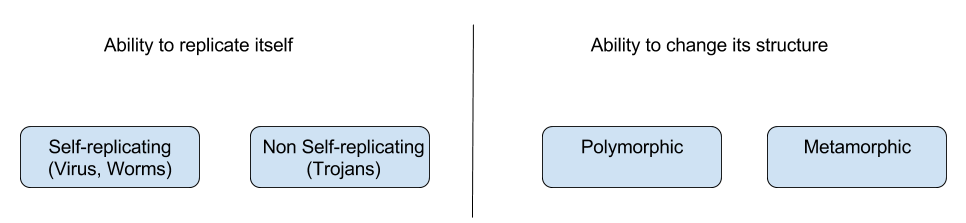
\includegraphics[scale=0.3]{figures/malware_type.png}
  \label{fig:malware_type}
  \end{figure}
  \item Different variants of same malware and hard to detect with signature based
\end{itemize}
\end{frame}

\begin{frame}[plain]{Growth of Malware}
  \begin{columns}
    \begin{column}{5cm}
      \begin{figure}[H]
        \begin{center}
          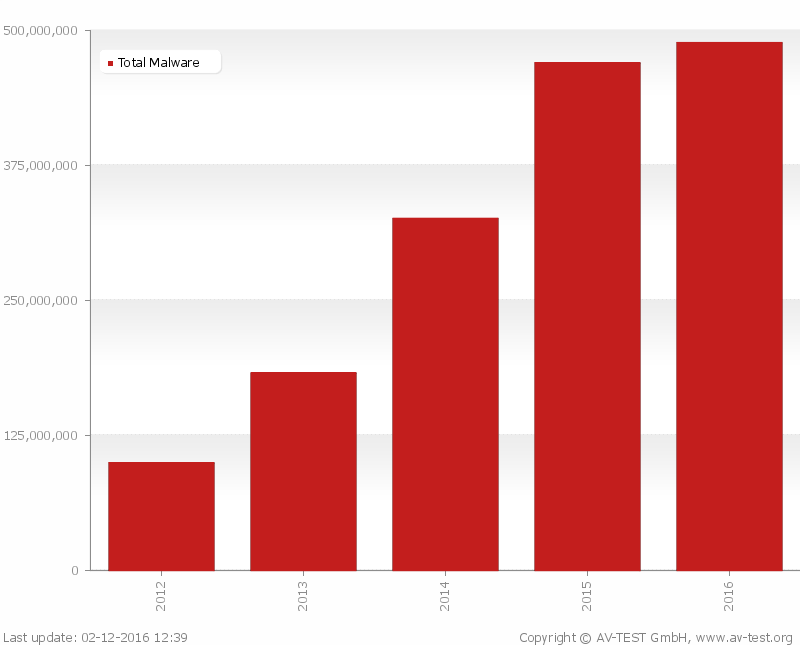
\includegraphics[scale=0.18]{figures/malware_all.png}
        \end{center}
      \end{figure}
    \end{column}
    \begin{column}{5cm}
      \begin{figure}[H]
        \begin{center}
          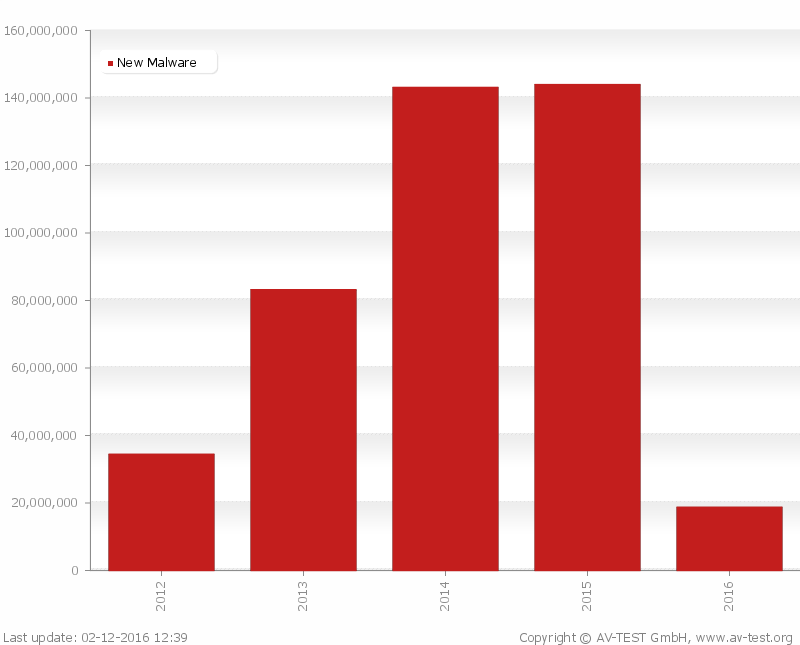
\includegraphics[scale=0.18]{figures/malware_new.png}
        \end{center}
      \end{figure}
    \end{column}
  \end{columns}
  \begin{itemize}
    % \item Malware authors are introducing new malware on daily basis to steal those valuable data and personal information and sell it illegally in the underground market.
    \item High rise, driven by monetary profit
    \item In 2006, 2.8 billion dollars in US and 9.3 billion euros in Europe
  \end{itemize}
\end{frame}
\begin{frame}[t]{Interference Between Malware Families}
  \begin{itemize}
    \item There has been some anecdotal evidences of feud between the malware families
    \item In 2004, NetSky vs Bagle and MyDoom trying to remove each other along with message of profanity
    \item In 2010, SpyEye vs Zbot with KillZeus feature
    \item In 2015, Shifu malware family with AV like feature
    \item remove/prevent the infection of another malware
    \item Increase their own profit?
  \end{itemize}
\end{frame}
\subsection{Problem Statement}
\label{sub:Problem Statement}
\begin{frame}[t]{Problem Statement}
\begin{itemize}
  \item The purpose of our research is to identify the existence of aforementioned behavioral interference between the malware families
  \item Dynamic aspect of modern malware, the inter-family relations, and their associated underground economy
  \item Environment-sensitive malware
  % \item The study will provide novel knowledge for understanding the dynamic aspect of modern malware, the inter-family relations, and their associated underground economy
  % \item This behavior is also a case for environment-sensitive malware
  % \item That is to say malware changing their behavior depending on different factors of their running environment, such as presence or absence of files, programs, or running services
\end{itemize}
\end{frame}

\section{Methodology}
\label{sec:Methodology}
% \begin{frame}[t]{Research Process}
% \begin{itemize}
% \item Get wide variety of malware samples
% \item Use heuristics and clustering to get the candidate pair list
% \item Run each candidate pair in malware analysis system (Anubis in our case)
% \item Analyze the log of analysis run to detect behavioral interference
% \end{itemize}
% \begin{figure}[h]
%     \centering
%     \scalebox{0.5}{\input{figures/overview.pdf_tex}}
% \end{figure}
% \end{frame}
% \begin{frame}[t]{Heuristics}
%   \begin{itemize}
%     \item Millions of malware samples collected over time by Anubis
%     \item Need to find candidate pairs from the dataset with probability of behavioral interference
%     \item Choose based on common resource such that one malware created the resource and another malware tried to delete the same resource, but with failure
%     \item Parsed behavioral profiles of malware to get the failed delete/access operations
%     \item Reverse index of resource to malware samples
%     \item Large number of possible pairs and inconsistent AntiVirus label lead to Clustering of malware sample
%   \end{itemize}
% \end{frame}
% \subsection{Clustering}
% \label{sub:Clustering}
% \begin{frame}[t]{Latent Dirichlet Allocation}
%   \begin{itemize}
%     \item Clustering of malware with respect to their behavioral profile
%     \item LDA\@: General probabilistic model for collection of discrete data such as text corpora
%     \item Does not depend on number of documents and its memory footprint is $O (words \times topics)$
%     \item Each malware is represented as document and their activities as words in document
%     \item Resource types, operations, and resource name were represented by numeric id
%     \item We had a good clustering result with high intra-distance and low inter-distance of clusters
%   \end{itemize}
% \end{frame}

% \subsection{Candidate Selection}
% \label{sub:Candidate Selection}
% \begin{frame}[plain]{Candidate Selection}
% \begin{algorithm}[H]
%   \small
%   \begin{algorithmic}[1]
%     \STATE$R$   = Set of all interesting resource
%     \STATE$A_r$ = Set of malware that creates a particular resource `r'
%     \STATE$B_r$ = Set of malware that delete/access (failed) particular resource `r'
%     \STATE$N$   = Maximum number of families to consider
%     \STATE$E$   = Set of all probable candidate
%     \STATE\ \textbf{function} C (j)
%       \STATE\hspace{\algorithmicindent} $c_j =$ cluster id that malware $j$ belongs to
%       \STATE\hspace{\algorithmicindent} \textit{Return} $c_j$
%     \STATE\ \textbf{end function}
%     % \Function\
%     % \EndFunction\
%     \FORALL{$r \in R$}
%       \IF{$|C(x_r): x \in A_r| > N \lor |C(y_r): y \in B_r| > N$}
%         \STATE\ \textbf{continue}
%       \ENDIF\
%       \FORALL{$(x_r,y_r) \in A_r \times B_r$}
%         \IF{$C(x_r) \neq(y_r)$}
%           \STATE$E\gets (x_r, y_r)$
%         \ENDIF\
%       \ENDFOR\
%     \ENDFOR\
%   \end{algorithmic}
% \end{algorithm}
% \end{frame}

% \subsection{Executing the Candidate Pair}
% \label{sub:Executing the Candidate Pair}
% \begin{frame}[t]{Packer/Unpacker}
%   \begin{itemize}
%     \item The candidate pairs had to be run together inside the Anubis system
%     \item We used the fact that addition of extraneous data would not affect the binary execution
%     \item `Unpacker' binary read itself from the behind
%     \item The `Packer' packs the candidate pair along with meta-information such as its size and time delay to Unpacker
%     \item The Unpacker then would create the malware sample and execute it with specified time delay inside Anubis
%   \end{itemize}
% \end{frame}

\section{Contribution}
\begin{frame}[t]{Contribution}
Our research will provide the following contributions:
\begin{itemize}
  \item Systematic study of interferences between malware families
  \item A novel approach to malware clustering based on malware behavior profiles
  \item An automated system that detects interfering malware samples on a large scale
\end{itemize}
\end{frame}

\section{Evaluation}
\label{sec:Evaluation}
\subsection{Experiment}
\label{sub:Experiment}
\begin{frame}[t]{List of Candidate Pairs}
\begin{columns}
\begin{column}{4.7cm}
\begin{itemize}
  \item Value of N (maximum family cutoff) in algorithm chosen to be 10
  \item File with the highest number of candidate pair and Process the lowest
  \item No candidate pair from resource type Job, Device, Driver
\end{itemize}
\end{column}
\begin{column}{5.3cm}
  \begin{tabular}{l l l l}
    \toprule
    Resource types & \#candidate pairs\\
    \midrule
    File & 213,171 \\
    Registry & 39,899 \\
    Sync & 7,781 \\
    Section & 2,786 \\
    Process & 54\\
    \bottomrule
    Total & 263,691\\
  \end{tabular}
\end{column}
\end{columns}
\end{frame}
\begin{frame}[t]{Experiment Setup}
  \begin{itemize}
    \item 7 Anubis instance
    \item Each instance emulates entire running PC with Windows XP Service Pack 3 as OS
    \item Uses Qemu and monitors process by invoking callback routine for every basic block executed in virtual processor
    \item Unpacker and Packer used to run the candidate pair
    \item 10 minutes as total run time of each candidate pair experiment
    \item 4 minute for each malware, and 2 minute to boot system
  \end{itemize}
\end{frame}
\subsection{Results}
\label{sub:Results}
\begin{frame}[t]{Result of Candidate Run}
  \resizebox{\columnwidth}{!}{%
  \begin{tabular}{l l l l}
    \toprule
    Resource types & \# tested pairs & \# true positive & prediction accuracy\\
    \midrule
    File & 5,000 & 1032& 20.64\%\\
    Registry & 5,000 & 731& 14.62\%\\
    Sync & 1,000 & 119& 11.9\%\\
    Section & 1,000 & 93& 9.3\%\\
    Process & 54 & 6& 11.11\%\\
    \bottomrule
    % Total & 263691\\
  \end{tabular}%
}
\begin{itemize}
  \item Highest Accuracy for File and Registry
  \item Lowest for Process
  \item Average accuracy rate $14.25\%$
\end{itemize}
\end{frame}
\begin{frame}{Some Examples}
  \begin{itemize}
    \item Artemis! vs Cosmu on resource \url{C:\\Old.exe}
    \item VB.CB vs Startpage.AI on resource \url{C:\\WINDOWS\\window.exe}
    \item KeyLogger vs OnlineGames on resource \url{C:\\windows\\system32\\svrchost.exe}
  \end{itemize}
\end{frame}
\section{Threats to Validity}
\begin{frame}{Threats to Validity}
  \begin{itemize}
    \item Different values of N would give different candidate pairs and different results
    \item Didn't deal with random resource name
    \item Total execution time 10 minutes
    \item Sequence of execution
    \item Semantics of Malware
  \end{itemize}
\end{frame}


\section{Conclusion and Future Work}
\begin{frame}{Conclusion}
  \begin{itemize}
    \item Behavioral interference between malware families exists
    \item Malware checks for the presence of resource created by other malware and deletes it
    \item Our system could detect such interfering malware with average accuracy rate of $14.25\%$
    \item In our dataset, Files and Registries were the most interfered resource and Process was the least
  \end{itemize}
\end{frame}
\begin{frame}{Future Work}
  \begin{itemize}
    \item Make the experiment more efficient to run multiple times with different parameters
    \item Research on other possible approaches to clustering
    \item In depth analysis (static) of positive pair to know the true semantics of malware
  \end{itemize}
\end{frame}
\begin{frame}[plain,c]{Questions}
  \begin{center}
    \Huge QUESTIONS???
  \end{center}
\end{frame}
\appendix
\begin{frame}[plain,fragile]{Reverse Index}
\begin{lstlisting}[numbers=none,language=bash,caption={Sort and join the reverse index}]
LANG=en_EN sort -t, -k 1,1 $file_name
LANG=en_EN join -t , -a1 -a2 $fn1 $fn2
\end{lstlisting}
\begin{lstlisting}[numbers=none,caption={Sample of reverse index created for File activity},label={lst:reverseindex}]
C:\mbr.exe,189524063,184501719,87504631,86763863
C:/DOCUME~1/ADMINI~1/LOCALS~1/Temp/telnet.exe,178046895,174206059,183601891,89650247
C:/DOCUME~1/ADMINI~1/LOCALS~1/Temp/1.jpg,161552035,116241803
\end{lstlisting}
\end{frame}
\begin{frame}[plain]{Unpacker}
\begin{figure}[H]
  \centering
  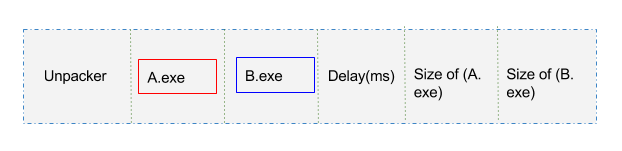
\includegraphics[scale=0.5]{figures/unpacker.png}
\caption{Structure of the Unpacker binary that would create the candidate pair and run them with delay.}
\label{fig:unpacker}
\end{figure}
\end{frame}
\begin{frame}[plain]{Inter and Intra Distance}
\begin{columns}
  \begin{column}{5cm}
    \begin{figure}[H]
      \begin{center}
        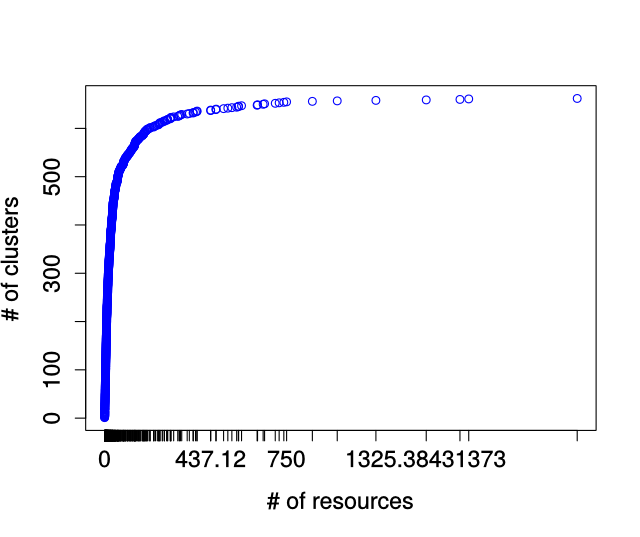
\includegraphics[scale=0.3]{figures/intra_clustered_common.png}
      \end{center}
      \captionsetup{font=small}
      \caption{ Graph showing cdf distribution of common resource between same family topic}
    \end{figure}
  \end{column}
  \begin{column}{5cm}
    \begin{figure}[H]
      \begin{center}
        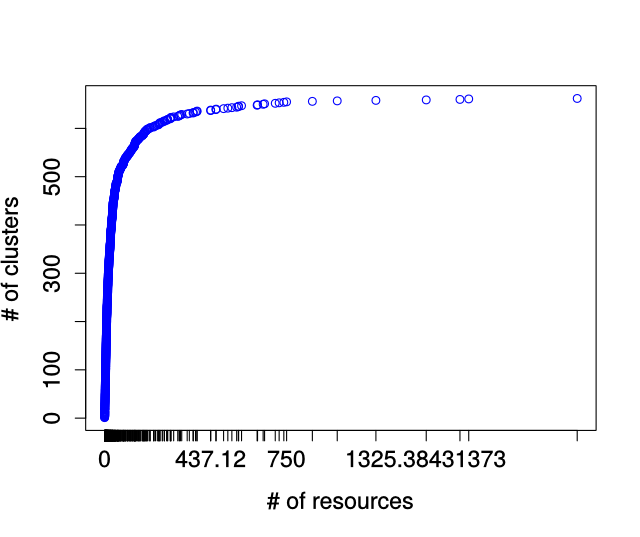
\includegraphics[scale=0.3]{figures/intra_clustered_common.png}
      \end{center}
      \captionsetup{font=small}
      \caption{ Graph showing cdf distribution of common resource between same family topic}
    \end{figure}
  \end{column}
\end{columns}
\end{frame}

\begin{frame}[plain]{Max Flow}
\begin{figure}[H]
  \centering
  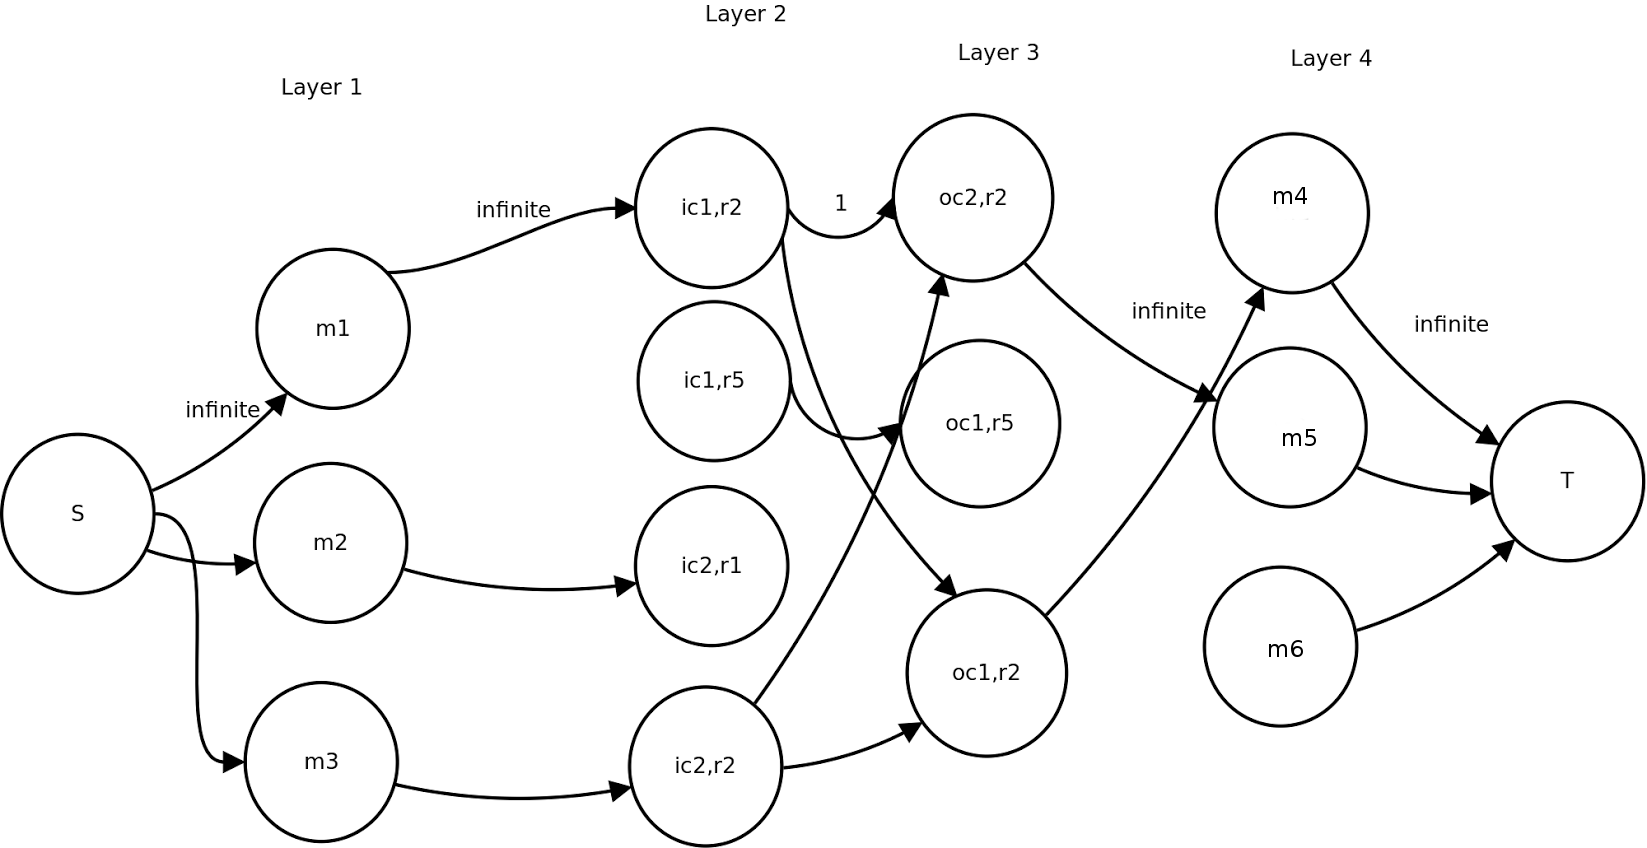
\includegraphics[scale=0.2]{figures/maxflow2.png}
  \caption[Max Flow]{Graph representing the max flow implementation}\label{fig:maxflow}
\end{figure}
\end{frame}

\begin{frame}[plain]{Heuristics}
\begin{figure}[H]
  \centering
  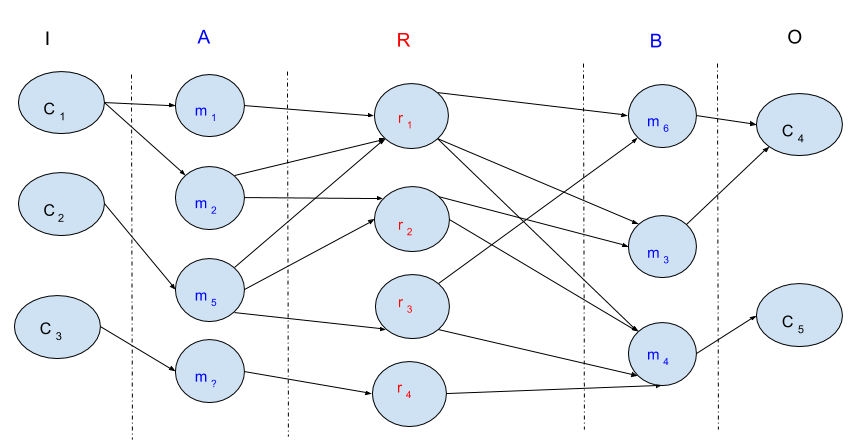
\includegraphics[scale=0.3]{figures/dhkheuristics.png}
  \caption[]{Heuristics approach to optimal malware pair selection}\label{fig:dhkheuristics}
  \centering
\end{figure}
\end{frame}
\end{document}
